% =============================================================================
% CAPÍTULO 1 — a raiz (AGENTS.md §6): a medida, o corte e o preço de fixar.
%
% O fracasso que o abre, com número na mão: a linha erguida no décimo terceiro pior
% dia dos últimos 252 pregões entrega 5,135% contra os 5% anunciados — parece
% cumprida —, mas o pior bloco de 60 dias tem 20 violações onde a promessa admitia
% 3, e nenhum dos 200 mundos que nunca mudam passou de 13.
%
% Medição: lab/experimentos/E01_promessa.ipynb. Figuras: figuras/E01_promessa_*.
% =============================================================================

\chapter{A medida, o corte e o preço}
\label{cap:medida}

\section{Uma pergunta de todo dia}

Quem carrega dinheiro aplicado faz, quase toda noite, a mesma pergunta: \emph{quanto eu
posso perder amanhã?} Não é pergunta de adivinho. É a pergunta que decide se a posição
cabe no bolso de quem a carrega --- e posição que não cabe no bolso é desmontada antes de
o mercado explicar por quê.

Toda tentativa de responder tem a mesma forma, e vale a pena escrevê-la em partes, porque
é dessas partes que este livro inteiro trata.

Primeiro escolhe-se \textbf{quantos dias olhar}. Depois olha-se o que aconteceu nesses
dias e \textbf{põe-se uma linha} num dos piores. Uma regra dessas, escrita por inteiro,
soa assim: \emph{o corte de hoje é o décimo terceiro pior dia dos últimos
\numCorteJanela{} pregões}. E o que ela pretende valer também se anuncia: \emph{não passo
daqui, dezenove dias em vinte} --- isto é, \numPromessaPct\% de violação.

Quatro palavras, com o mesmo sentido daqui em diante:

\begin{itemize}[leftmargin=1.5em]
  \item a \textbf{janela} é o pedaço do passado que a regra olha;
  \item o \textbf{corte} é onde a linha é posta dentro da janela;
  \item a \textbf{promessa} é a taxa de violação que se anuncia;
  \item a \textbf{entrega} é a taxa que de fato acontece.
\end{itemize}

A regra não é invenção deste livro: a linha posta no quantil dos piores dias é a medida de
risco mais usada em finanças, discutida e corrigida há décadas \cite{oconnell2026extreme}.
A pergunta deste capítulo é estreita, e é a primeira de todas: \emph{a entrega tem alguma
coisa a ver com a promessa?}

\section{O dado e a regra}

O dado sobre o qual tudo aqui é medido é o retorno de um dia para o outro. Com o preço de
hoje $p_t$ e o de amanhã $p_{t+1}$,
\[
  r_{t+1} = \log \frac{p_{t+1}}{p_t}.
\]

A razão do logaritmo aparece no exemplo mínimo: um preço que desce e volta ao lugar tem
retornos que somam zero.

\[ 100 \to 95: -0{,}0513; \qquad 95 \to 100: +0{,}0513; \qquad \text{queda de } 5\% \text{ pede alta de } 5{,}26\% . \] % numeros-ok: exemplo mínimo

Em porcentagem a volta também acontece, mas com números diferentes, porque porcentagem
multiplica onde o logaritmo soma. Somar, em vez de multiplicar, é o que permite acompanhar
o dia a dia sem perder o fio.

A série é o índice S\&P 500. % numeros-ok: nome próprio, não medição

São \numSerieDias{} pregões, de \numSerieInicio{} a \numSerieFim. Ela vem do
arquivo do projeto anterior, e o empréstimo fica declarado aqui --- o dado atravessa, e
todo número tirado dele é remedido neste capítulo.

Sobre ela, a regra tem duas decisões, e só duas. A \textbf{janela}: os
\numCorteJanela{} pregões anteriores a hoje. O \textbf{corte}: o décimo terceiro pior
deles. O corte de cada dia é erguido com os dias que já passaram e com nenhum outro, de
modo que a linha que se vê no gráfico estava lá antes de o dia acontecer. Um corte que
espiasse o futuro acertaria sempre e não valeria nada.

\section{A promessa parece cumprida}

Aplicada aos \numSerieDias{} pregões, a regra produz um corte novo a cada dia e uma
resposta por dia: o dia ficou abaixo da linha, ou não ficou. Nos \numEntregaDias{} dias em
que havia janela suficiente, a linha foi rompida \numEntregaViolacoes{} vezes.

\[
  \text{entrega} = \numEntregaTaxaPct\%, \qquad \text{promessa} = \numPromessaPct\%.
\]

A diferença é de um décimo de ponto percentual. Parece que funcionou.

Não funcionou, e o motivo não está no mercado: está na aritmética de erguer a linha.

\section{O corte assina a entrega}

\begin{proposicao}[a conta do corte]
\label{prop:conta}
Suponha que os $n$ dias da janela e o dia seguinte sejam $n+1$ valores de uma mesma lei
contínua, em qualquer ordem igualmente provável. Se o corte é o $k$-ésimo menor dos $n$
dias da janela, então a probabilidade de o dia seguinte ficar abaixo do corte é
$\dfrac{k}{n+1}$.
\end{proposicao}

\begin{proof}
Junte os $n+1$ valores e ponha-os em ordem crescente. Todas as ordens são igualmente
prováveis, então a posição do dia seguinte nessa fila é uniforme entre as $n+1$ posições.
O dia seguinte fica abaixo do corte exatamente quando ocupa uma das $k$ primeiras
posições, que são as ocupadas pelos $k$ menores da janela. Logo a probabilidade é
$k/(n+1)$.
\end{proof}

A lei ser contínua serve para que dias empatados tenham probabilidade zero, e a hipótese
de que todas as ordens são igualmente prováveis é a hipótese de que os dias não têm nada a
dizer uns sobre os outros --- que é justamente o que um mundo que muda viola. A proposição
não é a previsão do que vai acontecer; é o contraste contra o qual o que aconteceu se lê.

A proposição é um caso pequeno e exato de um viés conhecido: quantil estimado de uma
amostra não entrega a probabilidade que se anuncia, e o tamanho do erro depende do tamanho
da amostra \cite{taleb2020super}.

Com $n = \numCorteJanela$ e $k = \numCortePosto$, a conta dá
$\numCortePosto/(\numCorteJanela+1)$: \numCorteContaPct\%. Esse número não vem do mercado.
Vem da decisão de olhar \numCorteJanela{} dias e cortar no décimo terceiro. E a promessa
anunciada está fora do alcance desse corte --- o posto teria de cair entre dois dias, e
não existe o décimo terceiro dia e meio de um ano. Com \numCorteJanela{} pregões, as duas
taxas ao lado da promessa são \numCorteAlternativoPct\%, no décimo segundo, e
\numCorteContaPct\%, no décimo terceiro. Nenhuma das duas é \numPromessaPct\%.

Medimos, e o mercado entregou \numEntregaTaxaPct\% --- \numEntregaViolacoes{} rompimentos
em \numEntregaDias{} dias. É o que o corte assinou, com poucos milésimos de diferença.
Para saber se essa diferença diz alguma coisa, falta o único contraste que responde:
submeter um mundo em que nada muda exatamente à mesma rotina.

Sorteamos \numNuncaMudaMundos{} séries do tamanho da nossa, com retornos independentes e
sempre com a mesma lei, e aplicamos a cada uma a mesma regra. A entrega média desses
mundos foi \numNuncaMudaTaxaPct{} --- contra os \numCorteContaPct\% da conta. E o mundo
real entregou \numEntregaTaxaPct\%.

\emph{A média não distingue o mundo real de um mundo que nunca mudou.}

Este é o primeiro princípio do livro, e ele é desconfortável: a média de violações é uma
\textbf{propriedade do corte, não do mundo}. Não porque o mundo não apareça, mas porque o
corte já assinou o número antes de qualquer dado chegar. Quem lê só a média lê a própria
escolha e acredita estar lendo o mercado.

\section{O que a média não vê}

O mundo aparece em outro lugar, e o lugar é a \emph{forma} com que as violações chegam:
espalhadas pelo calendário, ou concentradas em pedaços. Para medir a forma, contamos
quantas violações caem em cada janela móvel de \numBlocoDias{} dias --- a isso chamamos um
\textbf{bloco} ---, e olhamos o bloco mais cheio. A promessa de \numPromessaPct\% admite
\numBlocoPrometido{} violações em \numBlocoDias{} dias.

A mediana dos blocos é \numBlocoMediana{}: na maior parte do tempo a linha aguenta mais do
que prometeu. O pior bloco tem \numBlocoPior{} violações, e termina em
\numBlocoPiorData. Onde a promessa admitia \numBlocoPrometido{}, aconteceram
\numBlocoPior.

Nos \numNuncaMudaMundos{} mundos que nunca mudam, o pior bloco de cada um teve, em média,
\numNuncaMudaPiorMedio{} violações, e o pior bloco de todos eles chegou a
\numNuncaMudaPiorBloco. Nenhum passou disso. A série real, com o mesmo tamanho e a mesma
rotina, chegou a \numBlocoPior.

\begin{figure}[htbp]
  \centering
  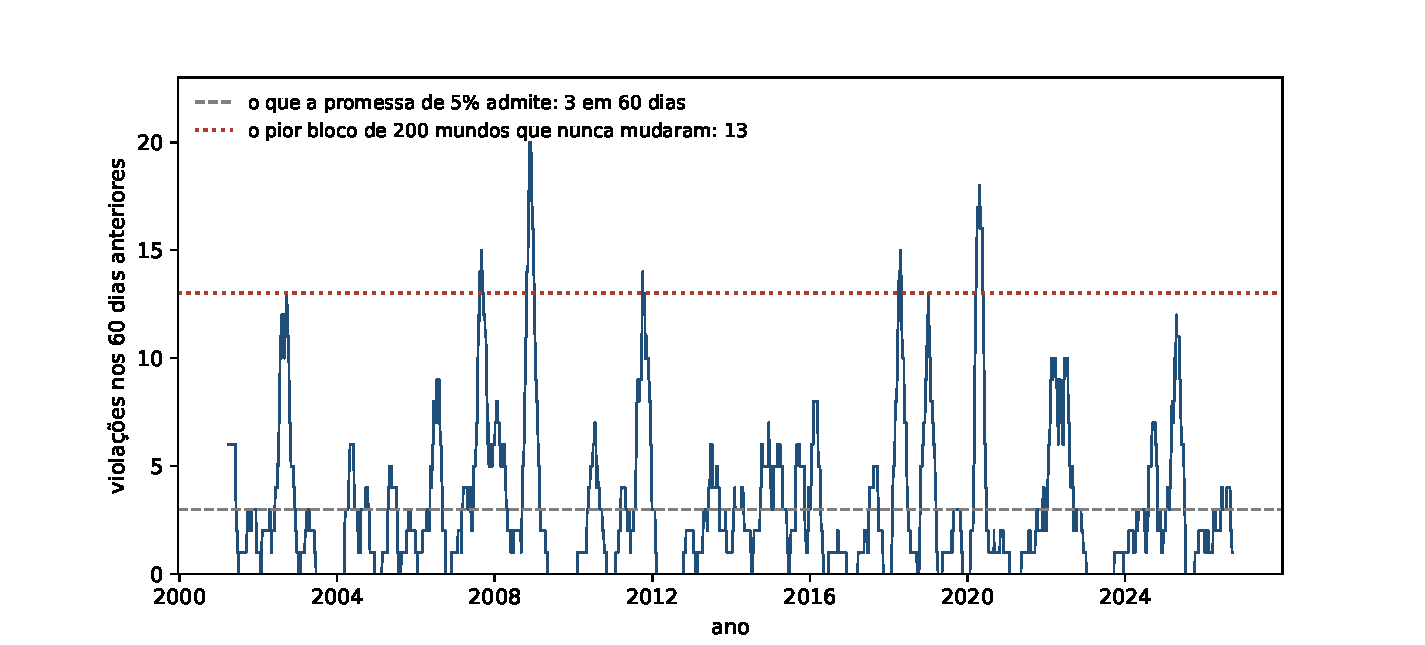
\includegraphics[width=\linewidth]{figuras/E01_promessa_1.pdf}
  \caption{Violações nos \numBlocoDias{} dias anteriores, dia a dia. A linha tracejada é o
    que a promessa de \numPromessaPct\% admite; a pontilhada é o pior bloco que apareceu
    em \numNuncaMudaMundos{} mundos que nunca mudam.}
  \label{fig:blocos}
\end{figure}

A figura mostra o que a média esconde: a série passa trechos longos colada na linha da
promessa e sobe, em surtos curtos, até cruzar a linha pontilhada. E os blocos têm data. O
teto dos mundos que nunca mudam é cruzado em \numEpisodiosAcimaDoTeto{} episódios
distintos, que ocupam \numBlocosAcimaDoTetoPct\% dos blocos medidos, em
\numEpisodiosAnos. Nem todos esses anos têm nome de crise, e todos aconteceram neste
mercado.

A leitura do bloco corrige ainda a primeira impressão: \numBlocoAcimaDoDobroPct\% dos
blocos passam do dobro da promessa. O que se promete não é o que se entrega, nem na maior
parte do tempo, nem nos piores pedaços --- é uma média entre os dois.

\section{O preço não desaparece: muda de endereço}

Se o corte assina a média, uma saída parece evidente: escolher outra janela. Vale a pena
tentar, e a tentativa é barata, porque é a mesma regra com outro número. Varremos a janela
de um mês a cinco anos, mantendo a promessa anunciada de \numPromessaPct\% e o bloco de
\numBlocoDias{} dias.

\begin{table}[htbp]
  \centering
  \begin{tabular}{rrrr}
    \hline
    janela & a conta do corte & a entrega & o pior bloco \\
    (pregões) & (\%) & (\%) & (violações) \\
    \hline
    \numCorteCurtoJanela & \numCorteCurtoContaPct & \numCorteCurtoTaxaPct & \numCorteCurtoPiorBloco \\
    \numCorteMedioJanela & \numCorteMedioContaPct & \numCorteMedioTaxaPct & \numCorteMedioPiorBloco \\
    \numCorteJanela & \numCorteContaPct & \numEntregaTaxaPct & \numBlocoPior \\
    \numCorteLongoJanela & \numCorteLongoContaPct & \numCorteLongoTaxaPct & \numCorteLongoPiorBloco \\
    \hline
  \end{tabular}
  \caption{A mesma regra com quatro janelas, a mesma promessa anunciada de
    \numPromessaPct\% e o mesmo bloco de \numBlocoDias{} dias. A coluna do meio é a conta
    da \cref{prop:conta}; a última é o pior bloco medido.}
  \label{tab:varredura}
\end{table}

As três colunas contam uma história só, e ela é a resposta deste capítulo.

A \textbf{conta do corte} obedece à promessa anunciada apenas na janela longa. Na janela
de um mês, o corte assina \numCorteCurtoContaPct\% --- quase o dobro dos
\numPromessaPct\% anunciados ---, e a razão é aritmética, não mercado: com poucos dias não
existe corte que produza \numPromessaPct\%.

A \textbf{entrega} acompanha a conta do corte nas quatro janelas, um pouco acima dela em
todas. Esse resto é a contribuição do mundo, e é pequeno. Encurtar a janela não deixa a
medida mais fina; torna a promessa mais caro do que se anunciou.

O \textbf{pior bloco} caminha no sentido oposto: \numCorteCurtoPiorBloco,
\numCorteMedioPiorBloco, \numBlocoPior, \numCorteLongoPiorBloco. Quanto mais longo o
passado que a linha olha, mais tempo ela leva para acompanhar o que mudou, e mais
violações cabem no pedaço ruim. Na janela de cinco anos o pior bloco chega a
\numCorteLongoPiorBloco. E, no extremo oposto, uma janela curta não compra bloco nenhum: o
pior bloco do mundo real, \numCorteCurtoPiorBloco, fica \emph{abaixo} do pior bloco de um
mundo que nunca muda, porque uma janela curta se move junto com o mercado --- e cobra o
preço na média.

\begin{figure}[htbp]
  \centering
  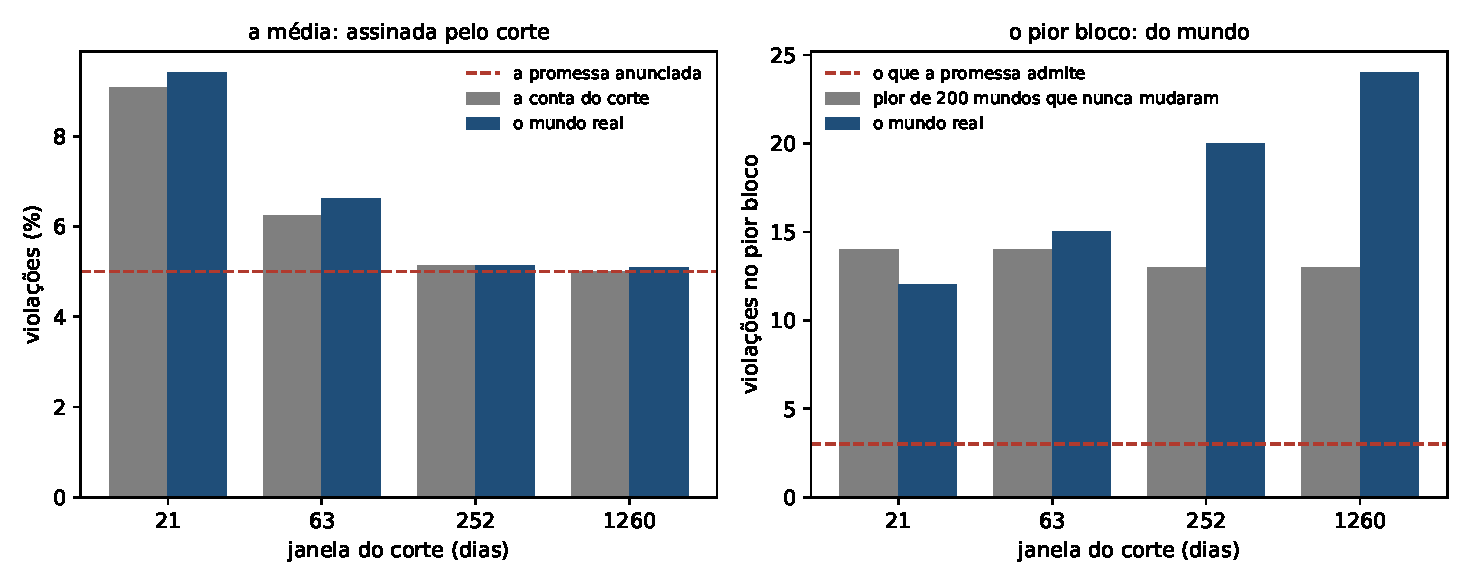
\includegraphics[width=\linewidth]{figuras/E01_promessa_2.pdf}
  \caption{As duas leituras, nas quatro janelas. À esquerda, a média: a conta do corte e o
    mundo real andam juntos. À direita, o pior bloco: o mundo real contra o pior dos
    \numNuncaMudaMundos{} mundos que nunca mudam.}
  \label{fig:duas}
\end{figure}

\emph{O preço de fixar não desaparece: muda de endereço.} Encurtar o corte cobra na média;
alongá-lo cobra no bloco. Não há janela em que a linha entregue o que a promessa anunciou
--- e a razão é a \cref{prop:conta}, que não deixa o mundo entrar na conta.

\section{O que fica}

Ficam três movimentos, e eles são o instrumento deste livro. Primeiro, \textbf{declarar o
corte}: a taxa que se assina não é a taxa que se anuncia, e a diferença é a conta da
\cref{prop:conta}. Segundo, \textbf{ler em bloco, não em média}: a média é assinada pelo
corte, e só o bloco responde pelo mundo. Terceiro, \textbf{varrer o corte}: o preço não
some quando se troca de janela --- ele se muda, e saber para onde ele foi é a decisão.

E fica um fracasso, visível e sem resposta aqui. Um corte fixo supõe que o pedaço de
passado que ele olha se parece com o pedaço que vem. A série deste capítulo não se parece
consigo mesma: passa meses colada na linha e depois rompe a linha \numBlocoPior{} vezes em
\numBlocoDias{} dias. Se os blocos têm data, alguma coisa no mundo não é fixa, e a média
não é o instrumento que a vê.

A próxima pergunta, então, não é qual janela escolher --- é \emph{que formas a mudança
tem}: se ela chega pela média, pela cauda, pela dependência entre coisas que antes andavam
separadas, ou pelo calendário. Responder exige um instrumento novo: um orçamento de erro
declarado, contra o qual cada mudança possa ser cobrada. É para lá que este livro vai
agora.
